%%%%%%%%%%%%%%%%%%%%% chapter.tex %%%%%%%%%%%%%%%%%%%%%%%%%%%%%%%%%
%
% esempio di capitolo
%
% Usare questo  file come template per il vostro documento.
%
%%%%%%%%%%%%%%%%%%%%%%%% Springer-Verlag %%%%%%%%%%%%%%%%%%%%%%%%%%

\chapter{Rotazioni}
\label{Rotazioni} % Fornire sempre un'unica label
% usare \chaptermark{}
% per alterare o aggiustare l'intestazione del capitolo nella running head

Trasformazioni di un vettore utilizzando angoli di rotazione o quaternioni.
\section{Matrice di rotazione}
Con la matrice di rotazione $[_1^0A]$ si intende la matrice che trasforma le coordinate del vettore r espresse nel riferimento ruotato 1 ${^1r}$ , nel sistema di riferimento 0. \newline In generale sarà presente anche una traslazione tra i due riferimenti, ragion per cui compare un termine di traslazione d:
\begin{equation}
\label{eq:1.1}
\left\{^0r\right\} = \left[_1^0A\right]\left\{^1r\right\} + \left\{^0d\right\}
\end{equation}

\begin{figure}[h!]
\centering
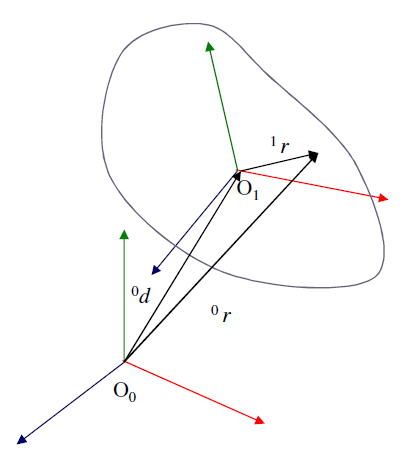
\includegraphics[height=6cm]{rotation_1.png}
\caption{Trasformazione delle coordinate di un punto}
\label{fig:1.1}
\end{figure}
La matrice di rotazione $\in \mathbb{R}^{3x3}$ per cui è definita da 9 elementi, tuttavia per calcolarla bastano 3 o 4 parametri a seconda che si utilizzino gli angoli di rotazione o i quaternioni.
\section{Angoli di Eulero}
La matrice relativa alla rotazione attorno ad un asse del riferimento può essere ricavata con calcoli trigonometrici. Poiché una qualsiasi rotazione può essere espressa come una successione di 3 rotazioni attorno a 3 assi distinti è possibile risalire alla coordinata del punto nel riferimento 3 arbitrariamente ruotato con un prodotto di matrici:
\begin{equation}
\label{eq:1.2}
\left\{^0r\right\} = \left[_1^0A\right]\left[_2^1A\right]\left[_3^2A\right]\left\{^3r\right\}
\end{equation}
La scelta della sequenza di assi di rotazione non è univoca. Per questo si sono diffuse differenti convenzioni. La più diffusa è quella degli angoli di Eulero:
\begin{figure}[h!]
\centering
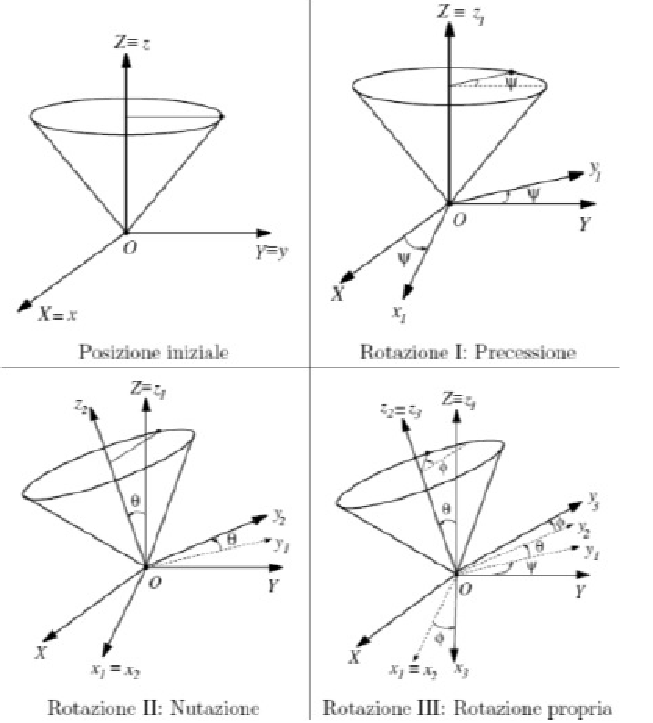
\includegraphics[height=10cm]{euler_angles.pdf}
\caption{Angoli di Eulero}
\label{fig:1.2}
\end{figure}
L'utilizzo della matrice di rotazione fornisce formule dirette per il calcolo di posizioni, velocità ed accelerazioni nel riferimento fisso a patto di conoscere angoli e velocità angolari dei sistemi di riferimento solidali ai corpi del sistema. Emergono tuttavia due limiti a questo approccio: \begin{itemize}
\item L'ordine di applicazione degli angoli di rotazione dà luogo a configurazioni finali differenti (d'altronde il prodotto tra matrici non è commutativo). L'influenza dell'ordine di applicazione degli angoli ha portato diversi enti ad adottare diverse convenzioni.
\item Il limite maggiore di questo approccio tuttavia è l'emergere di singolarità nella soluzione del problema inverso; ovvero qualora si vogliano trovare gli angoli a partire dalla matrice, problema molto comune nelle applicazioni robotiche. Formalmente, esprimendo con x', y' e z' i versori lungo gli assi del riferimento mobile (ovviamente rispetto a quello fisso), si devono eguagliare elemento per elemento le matrici
\[ \begin{bmatrix}   \\ x'& y'&z' \\ \text{ } \end{bmatrix} = \begin{bmatrix}
a_{11} & a_{12} & a_{13} \\ a_{21} & a_{22} & a_{23} \\ a_{31} & a_{32} & a_{33}\end{bmatrix} \]
Con: \qquad $a_{33} = cos\theta,\qquad a_{32} = -sin\theta cos\phi \qquad$ ecc... \newline
È evidente che in corrispondenza di certi angoli si riscontrano singolarità ad è impossibile risolvere il sistema di 9 equazioni. Questo ha anche un riscontro pratico detto blocco cardanico o \textit{gimbal lock}: una sospensione cardanica con 3 cerniere con lo scopo di isolare un oggetto dalle rotazioni del telaio in certe configurazioni non permette più rotazioni arbitrarie, di fatto bloccando alcune rotazioni.  
\end{itemize}

\section{Quaternioni}
Per questa ragione si utilizzano 4 parametri, descrivendo le rotazioni tramite quaternioni. Si evitano così le singolarità nella cinematica inversa, l'utilizzo di funzioni trigonometriche per la soluzione del sistema ed il problema dell'arbitrarietà della sequenza di rotazioni.
In Generale un quaternione è un elemento scrivibile come $ \overline{q} = a + bi + cj+ ck$ con $i^2=j^2=k^2 = ijk -1$. \newline Il quaternione descrive una rotazione di un angolo $\theta$ attorno ad un versore u come in figura \ref{fig:1.3}.

La rotazione di un angolo $\theta$ attorno ad un versore di componenti ${a, b, c}$ è quindi decritta dal quaternione
\begin{equation} 
    \overline{q} = cos\frac{\theta}{2} + (ai + bj + ck)sin\frac{\theta}{2}
\end{equation}{}

Tramite l'utilizzo dei quaternioni si può esprimere:
\begin{itemize}
\item La cinematica diretta \begin{equation}
\label{eq:1.3}
(0, v') = \overline{q}(0,v)\overline{q}^*\end{equation}
Con (0,v) vettore di 4 elementi e $\overline{q}^*$ coniugato di $\overline{q}$
\item La cinematica inversa: \begin{equation}
\label{eq:1.4}
(0, v) = \overline{q}^*(0,v')\overline{q}\end{equation}
\item Rotazioni successive :
\begin{equation} 
    \overline{q} = \overline{q}_2 \overline{q}_1 
\end{equation}{}
\item La matrice di rotazione A:
\begin{equation}\left[A(q)\right] = \left[F(q)_+\right]\left[F(q)_-\right]^T \label{eq:1.5}\end{equation}
Con 
\begin{equation} \label{eq:1.6} \left[F(q)_+\right]\ = \begin{bmatrix}
+q_1 & +q_0 & -q_3 & +q_2 \\ +q_2 & +q_3 & +q_0 & -q_1 \\ +q_3 & -q_2 & +q_1 &+q_0\end{bmatrix}
\end{equation}
\begin{equation} \label{eq:1.7} \left[F(q)_-\right]\ = \begin{bmatrix}
+q1 & +q_0 & +q_3 & -q_2 \\ +q_2 & -q_3 & +q_0 & +q_1 \\ +q_3 & +q_2 & -q_1 &+q_0\end{bmatrix}
\end{equation}
\item Velocità in funzione di $ \dot{\overline{q}}$ e viceversa
\begin{equation} \label{eq:1.8}
\dot{\overline{q}} = \frac{1}{2}\left[F(q^*)_-\right]\overrightarrow{\omega}_0 = \frac{1}{2}\left[F(q^*)_+\right]\overrightarrow{\omega}_l\end{equation}
\begin{equation} \label{eq:1.9}
\overrightarrow{\omega}_0 = 2\left[F(q^*)_-\right]\dot{\overline{q}}\end{equation}
\begin{equation} \label{eq:1.10}
\overrightarrow{\omega}_l = 2\left[F(q^*)+-\right]\dot{\overline{q}}\end{equation}
\item Accelerazione angolare in funzione di $\ddot{\overline{q}}$ e viceversa
\end{itemize}
\begin{figure}[h!]
\centering
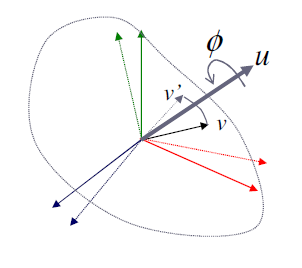
\includegraphics[height=5cm]{quaternion_def.png}
\caption{Trasformazione delle coordinate di un punto}
\label{fig:1.3}
\end{figure}




%
